\documentclass{beamer}
\usetheme{Boadilla}
\usepackage[compat=1.1.0]{tikz-feynman}
\usepackage{subcaption}

\title{My Presentation Title}
\author{Abigail McIntosh}
\institute{University of Sussex}
\date{\today}

\begin{document}

\begin{frame}
  \titlepage
\end{frame}

\begin{frame}{Outline}
  \tableofcontents
\end{frame}

\section{Section 1}
\subsection{Subsection 1.1}

% ========== TOP INTRODUCTION ==========
\begin{frame}{Top Quark}
  \begin{itemize}
    \item Heaviest known elementary particle ($m_t = 172.76 \pm 0.3$ GeV).
    \item Yukawa coupling $y_t \sim 1$, largest of all fermions.
    \item Short lifetime ($\tau \sim 5 \times 10^{-25}$ s), decays before hadronisation.
    \item Main production mechanisms:
    \begin{itemize}
      \item Pair production via strong interaction.
      \item Single top production via electroweak interaction (three channels).
      \item Associated production with other particles.
    \end{itemize}
    \item Plays large role in electroweak symmetry breaking and sensitive to BSM physics.
    \item LHC is a top factory.
  \end{itemize}
\end{frame}


% ========== TOP PAIR PRODUCTION ==========
\begin{frame}{$t\bar{t}$ Production}
  \begin{itemize}
    \item Dominant production mechanism at LHC.
    \item Mediated by strong interaction.
    \item Produced by either gluon-gluon fusion (90\%) or quark-antiquark annihilation (10\%).
  \end{itemize}
\end{frame}


% ========== SINGLE TOP PRODUCTION ==========
\begin{frame}[fragile]{Single Top Production}
  \begin{itemize}
    \item Charged-current electroweak process.
    \item Three production channels:
    \begin{itemize}
      \item $t$-channel: $q b \rightarrow q' t$
      \item $s$-channel: $q \bar{q}' \rightarrow t \bar{b}$
      \item $W$-associated production ($tW$): $g b \rightarrow t W$
    \end{itemize}
  \end{itemize}
  \begin{figure}[htbp]
    \centering
    % ========== t-channel ==========
    \begin{subfigure}[b]{0.31\textwidth}
      \centering
      \resizebox{\textwidth}{!}{%
      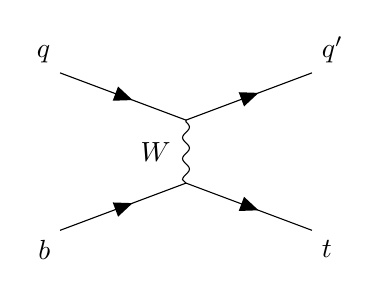
\begin{tikzpicture}
          \begin{feynman}
            \coordinate (a)  at (0, 0.4);
            \coordinate (b)  at (0, -0.4);
            \coordinate (f1) at (-1.6, 1.0);
            \coordinate (f3) at (1.6, 1.0);
            \coordinate (f2) at (-1.6, -1.0);
            \coordinate (f4) at (1.6, -1.0);

            \draw [fermion] (f1) node[above left] {\(q\)} -- (a);
            \draw [fermion] (a) -- (f3) node[above right] {\(q'\)};
            \draw [boson]   (a) -- node[left=2pt] {\(W\)} (b);
            \draw [fermion] (f2) node[below left] {\(b\)} -- (b);
            \draw [fermion] (b) -- (f4) node[below right] {\(t\)};
          \end{feynman}
      \end{tikzpicture}%
      }
      \caption{$t$-channel}
      \label{subfig:tchan}
    \end{subfigure}\hfill%
    % ========== s-channel ==========
    \begin{subfigure}[b]{0.31\textwidth}
      \centering
      \resizebox{\textwidth}{!}{
        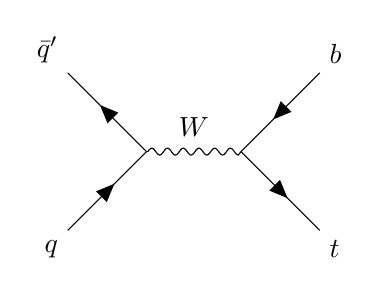
\begin{tikzpicture}
          \begin{feynman}
            \coordinate (a)  at (-0.6, 0);
            \coordinate (b)  at (0.6, 0);
            \coordinate (f1) at (-1.6, 1.0);
            \coordinate (f3) at (1.6, 1.0);
            \coordinate (f2) at (-1.6, -1.0);
            \coordinate (f4) at (1.6, -1.0);

            \draw [fermion] (a) -- (f1) node[above left] {\(\bar{q}'\)};
            \draw [fermion] (f2) node[below left] {\(q\)} -- (a);
            \draw [boson]   (a) -- node[above=2pt] {\(W\)} (b);
            \draw [fermion] (f3) node[above right] {\(b\)} -- (b);
            \draw [fermion] (b) -- (f4) node[below right] {\(t\)};
          \end{feynman}
        \end{tikzpicture}%
      }
      \caption{$s$-channel}
      \label{subfig:schan}
    \end{subfigure}\hfill%
    % ========== tW-channel ==========
    \begin{subfigure}[b]{0.31\textwidth}
      \centering
      \resizebox{\textwidth}{!}{
        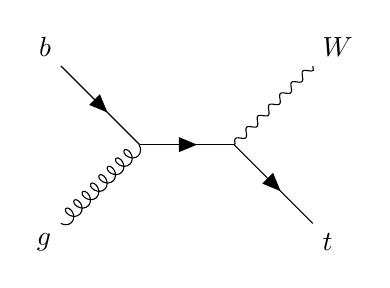
\begin{tikzpicture}
          \begin{feynman}
            \coordinate (a)  at (-0.6, 0);
            \coordinate (b)  at (0.6, 0);
            \coordinate (f1) at (-1.6, 1.0);
            \coordinate (f3) at (1.6, 1.0);
            \coordinate (f2) at (-1.6, -1.0);
            \coordinate (f4) at (1.6, -1.0);

            \draw [fermion] (f1) node[above left] {\(b\)} -- (a);
            \draw [gluon]   (f2) node[below left] {\(g\)} -- (a);
            \draw [fermion] (a) -- (b);
            \draw [boson] (b) -- (f3) node[above right] {\(W\)};
            \draw [fermion] (b) -- (f4) node[below right] {\(t\)};
          \end{feynman}
        \end{tikzpicture}%
      }
      \caption{$tW$-channel}
      \label{subfig:twchan}
    \end{subfigure}
    \caption{Feynman diagrams for single top production channels.}
    \label{fig:single-top-diagrams}
    \end{figure}
\end{frame}


% ========== ASSOCIATED TOP PRODUCTION ==========
\begin{frame}{Associated Top Production}
  \begin{itemize}
    \item Top quarks can also be produced in association with other particles, such as:
    \begin{itemize}
      \item $t\bar{t}W$ (top quark pair with W boson)
      \item $t\bar{t}Z$ (top quark pair with Z boson)
      \item $t\bar{t}\gamma$ (top quark pair with photon)
      \item $t\bar{t}H$ (top quark pair with Higgs boson)
    \end{itemize}
  \end{itemize}
\end{frame}

\begin{frame}{$t\bar{t}\gamma$ Production}
  \begin{itemize}
    \item Probes coupling between top quark and photon.
  \end{itemize}
  
\end{frame}

\end{document}